
%(BEGIN_QUESTION)
% Copyright 2006, Tony R. Kuphaldt, released under the Creative Commons Attribution License (v 1.0)
% This means you may do almost anything with this work of mine, so long as you give me proper credit

A simple form of electronic pressure transmitter could be made with a bourdon tube and a {\it differential capacitor}:

$$\includegraphics[width=15.5cm]{i00184x01.eps}$$

Explain how this instrument works, what type of electrical output signal it generates (e.g. current, voltage, resistance, etc.), and what polarity (if any) that output signal has.

\underbar{file i00184}
%(END_QUESTION)





%(BEGIN_ANSWER)

Hint: although it may not look like it at first, the two resistors form a {\it bridge circuit} with the differential capacitor.

%(END_ANSWER)





%(BEGIN_NOTES)

The output is an AC voltage, the magnitude of which is proportional to dielectric position, which in turn is proportional to applied pressure.

This particular instrument design would probably not be very practical unless the output voltage detector circuit were located very close to the bridge components so as to reduce parasitic capacitance(s).

\vskip 10pt

It might be good to review this formula with your students in discussing the operation of this capacitance-based instrument:

$$C = {\epsilon A \over d}$$

\noindent
Where,

$C =$ Capacitance in Farads

$\epsilon =$ Permittivity of dielectric (absolute)

$A =$ Conductor area, in square meters

$d =$ Separation distance, in meters

%INDEX% Measurement, pressure: differential capacitor as bourdon tube sensor

%(END_NOTES)


